\begin{figure*}[tb]
	\begin{minipage}[b]{.8\textwidth}
		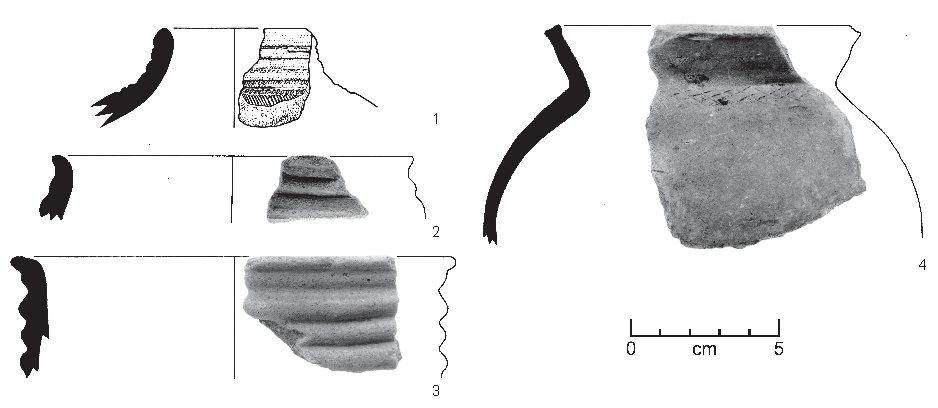
\includegraphics[width=\textwidth]{fig/BBL-Typen.pdf}
	\end{minipage}\hfill
	\begin{minipage}[b]{.2\textwidth}
		\caption{Bobulu-Gruppe: Typvertreter.\\1:~Taf.~25.13; 2:~Taf.~5.3; 3:~Taf.~5.4; 4:~Taf.~6.4.}
		\label{fig:BBL_Typverteter}
	\end{minipage}
\end{figure*}

\subsubsection{Bobulu-Gruppe}\label{sec:BBL-Gr}

Die Bobulu-Gruppe beschreibt insgesamt 62~GE aus Oberflächensurveys entlang des mittleren \mbox{Ubangi}. 34~GE bilden den Grundstock für die Beschreibung dieser Stilgruppe, während die übrigen 28~GE nur unter Vorbehalt als Teil der Bobulu-Gruppe angesprochen werden konnte. Diese Unsicherheit liegt in der Tatsache begründet, dass bis auf eine GE, die bei Grabungen in Maluba am Lua gefunden wurde (Fpl.~230; Kat.-Nr.~1), keines der Stücke aus einem geschlossenen oder stratifizierten Kontext stammt.\footnote{Die formale Ansprache der Bobulu-Gruppe basiert in Teilen auf den Surveyfunden aus der eponymen Fundstelle Bobulu am \mbox{Ubangi} (Fpl.~198). Komplex BBL~85/102 wurde im Gelände als \enquote{Konzentration mehrerer Gefäße beziehungsweise Gefäßfragmente} beschrieben (Feldbuch \textsc{Eggert} 15.08.1985). Der Bereich maß etwa 1,2\,m im Durchmesser und war 0,2\,m mächtig.} Die ausschließlich aus Surveys stammenden GE der Bobulu-Gruppe sind größtenteils kleiner als 70\,$\times$\,70\,mm (75\,\%). Größere Fragmente ließen sich nur selten im Fundgut nachweisen.

\paragraph{Technologische Merkmale}\hspace{-.5em}|\hspace{.5em}%
Die Scherben weisen regelhaft mittlere (34\,\%) bis hohe (37\,\%) Anteile nichtplastischer Partikel auf, vornehmlich heterogene Quarzsande, aber auch vereinzelt Glimmer und Fragmente von lateritähnlichem Gestein. Die \textit{Fabrics} der Bobulu-Keramik zeigen die bereits bei anderen Stilgruppen aus dem Bereich des \mbox{Ubangi} und Lua beobachtete Heterogenität. Bestimmt wird die Keramik der Bobulu-Gruppe von \textit{Fabrics} der Typen 3a (24\,\%), 4a (16\,\%) und 5c (11\,\%). Zu je etwa 10\,\% sind auch noch die \textit{Fabrics} 4c sowie 7d vertreten. Ein großer Teil der Stücke zeigt die Nutzung weißbrennender Tone (38\,\%) an, während nur wenige Stücke aus rotbrennenden Tonen (17\,\%) gefertigt wurden. Das Gros der Stücke weist überdies ein Farbspektrum auf, welches vor allem auf schwarz-, grau- und beige-Tönen basiert. Die Oberflächen der Stücke sind regelhaft glatt oder nur leicht rau. Die Wandungsdicke der Keramik der Bobulu-Gruppe liegt im Mittel bei 6,4\,mm.

\paragraph{Formen}\hspace{-.5em}|\hspace{.5em}%
Das Spektrum an Gefäßformen innerhalb der unter der Bobulu-Gruppe zusammengefassten GE weist eine auffällige Heterogenität auf. Am häufigsten ließen sich flache Gefäße mit geschweifter Wandung (Typ~E; 33\,\%) sowie Gefäße mit stark konvexer Wandung ohne ausgeprägten Halsbereich (Typ~D; 27\,\%; Abb.~\ref{fig:BBL_Typverteter}.4) beobachten. Ebenfalls vertreten sind aber auch Gefäße mit leicht konvexer Wandung und ausgeprägtem Halsbereich (Typ~C; 15\,\%), hohe (Typ~B; 9\,\%) und flaschenförmige Gefäße (Typ~A; 9\,\%) sowie Schalen mit konvexer Wandung und einbiegendem Rand (Typ~H; 6\,\%). Aufgrund der starken Fragmentierung der GE aus den Oberflächensurveys ließ sich jedoch nur bei knapp der Hälfte aller Stücke die Gefäßform sicher ansprechen. Die Gefäßwandungen sind fast ausschließlich konvex oder stark konvex ausgeführt (Abb.~\ref{fig:BBL_Typverteter}; Taf.~6.3). Die Ränder zeigen größtenteils eine spitze Randlippe (54\,\%). Deutlich seltener ließen sich runde (12\,\%) oder gerade abgestrichene Randlippen beobachten (12\,\%). Parallele, zylinderförmige Ränder sind die am häufigsten beobachtete Randform (A1; 26\,\%; Abb.~\ref{fig:BBL_Typverteter}.1; Taf.~5.10). Des Weiteren finden sich konkav ausbiegende (B2; 10\,\%) sowie kurze, konkav ausbiegende Ränder (B2.1; 17\,\%; Abb.~\ref{fig:BBL_Typverteter}.2; Taf.~5.8). Etwa gleich häufig kommen gerade ausbiegende Ränder (B1; 13\,\%; Abb.~\ref{fig:BBL_Typverteter}.4) sowie kurze, ausbiegende Ränder (B1.1; 10\,\%) vor. Seltener ließen sich konvex einbiegende Ränder beobachten (C3; 4\,\%; Taf.~6.3). Ein charakteristisches Element der Keramik der Bobulu-Gruppe ist das häufige Auftreten von Zylinderhälsen (68\,\%; Abb.~\ref{fig:BBL_Typverteter}.2--3; Taf.~5.8; 5.10). Deutlich seltener ist der Halsbereich der Gefäße überhaupt nicht ausgearbeitet (14\,\%; Abb.~\ref{fig:BBL_Typverteter}.4). Die Schulterbereiche sind größtenteils konvex (70\,\%; Abb.~\ref{fig:BBL_Typverteter}.1, 4) und nur selten gerade (30\,\%; Taf.~5.8). Bei keiner der Bobulu-Gruppe zugeordneten GE konnte die Ausformung des Gefäßbodens beobachtet werden.

\begin{figure*}[p]
	\centering
	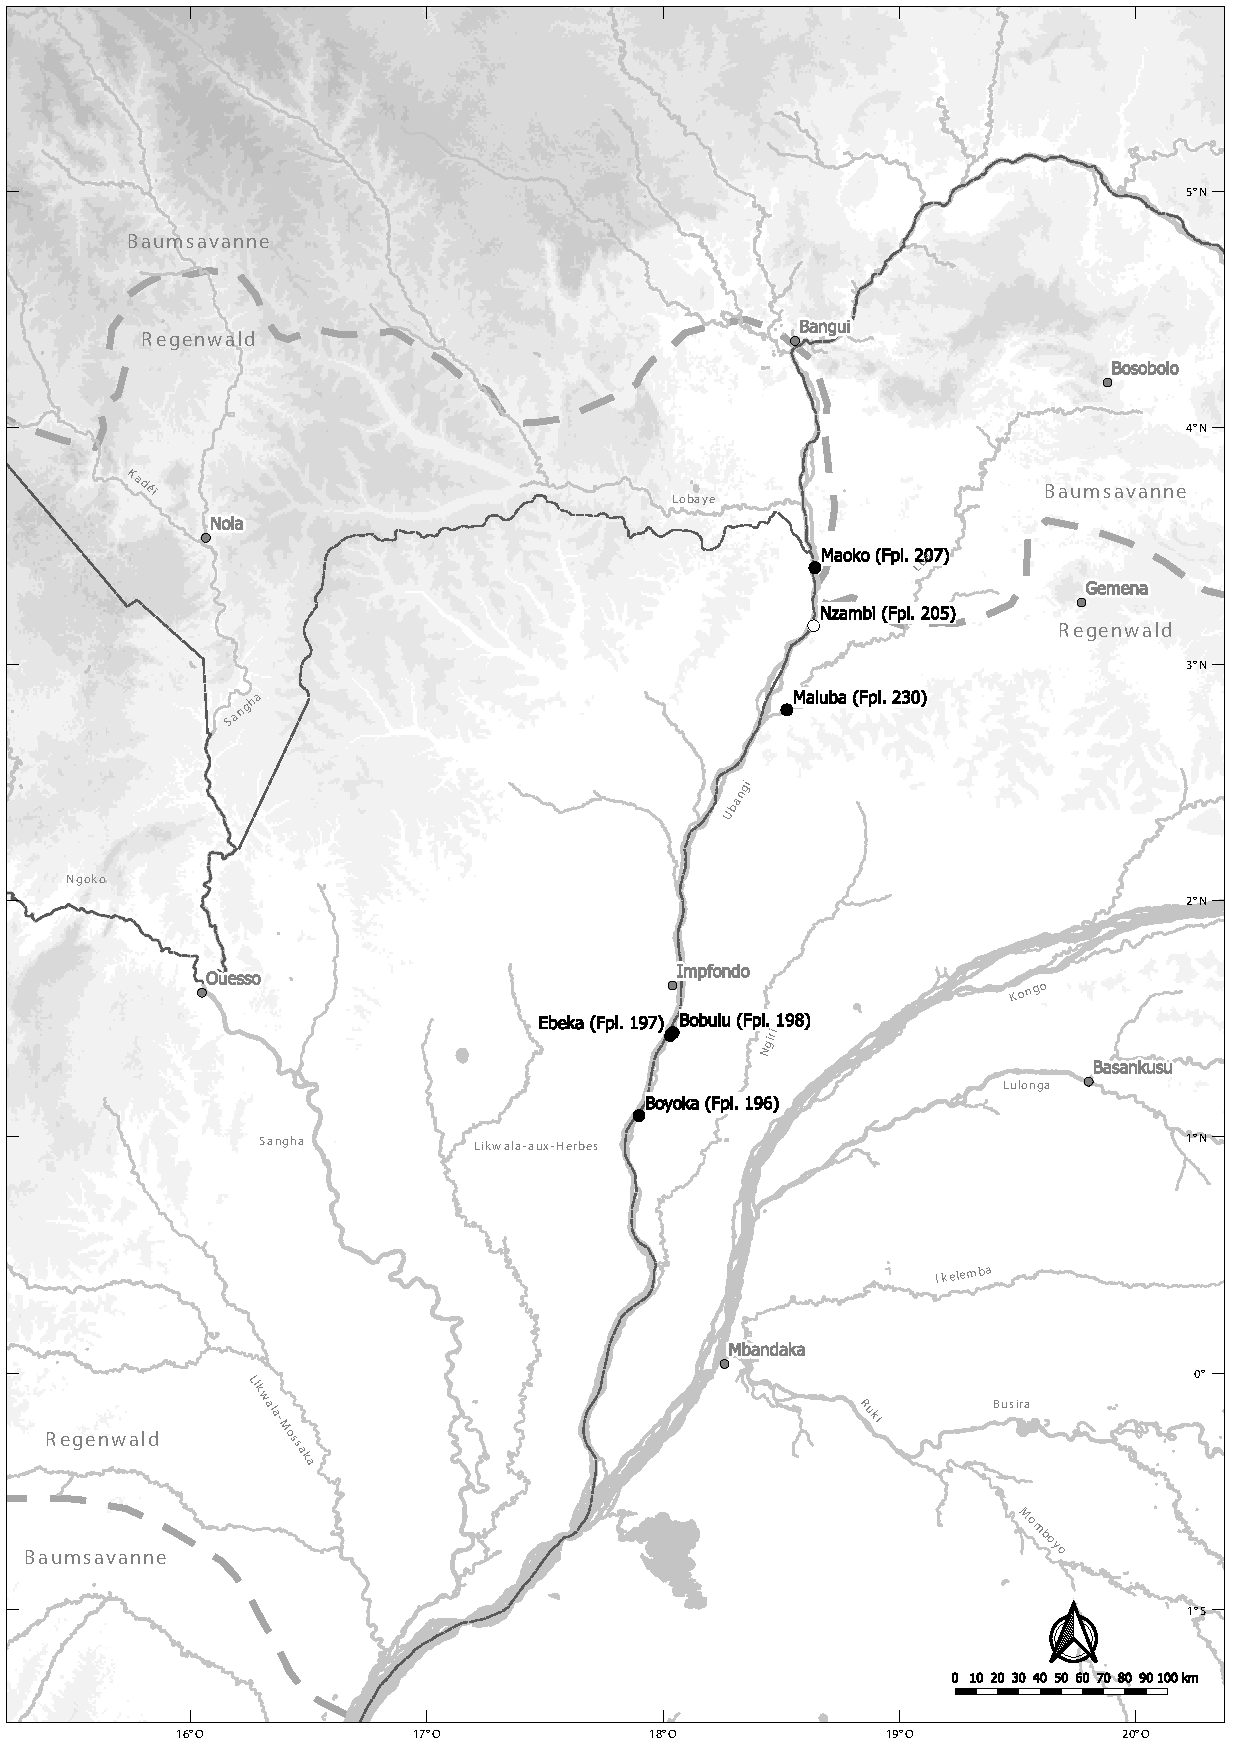
\includegraphics[width=\textwidth]{fig/BBL_Verbreitung.pdf}
	\caption{Bobulu-Gruppe: Verbreitung.}
	\label{fig:BBL_Verbreitung}
\end{figure*}

\paragraph{Verzierungen}\hspace{-.5em}|\hspace{.5em}%
Ein grundsätzliches Charakteristikum der Bobulu-Keramik ist ihre tendenzielle Verzierungsarmut. Die Hälfte aller beobachteten Verzierungselemente sind einfache Bündel aus horizontalen Rillen (Tab.~\ref{tab:Verzierungselemente}: 02.1). Insbesondere die Ränder und Halsbereiche weisen regelhaft eine Verzierung aus umlaufenden, tiefen, im Profil u-förmigen horizontalen Riefen auf (Abb.~\ref{fig:BBL_Typverteter}.1--3; Anlage~4\subref{fig:BBL_Verz}). Vereinzelt finden sich auf GE der Bobulu-Gruppe auch vegetabilische Rouletteverzierungen (Tab.~\ref{tab:Verzierungselemente}: 21.1--3), die zusammen etwa 6\,\% aller Verzierungselemente ausmachen und vor allem im Schulter- sowie Bauchbereich von Gefäßen zu beobachten sind (Anlage~4\subref{fig:BBL_Verz}). Schnitzroulette wurde nicht beobachtet. Im Bereich der Gefäßschultern lassen sich in einigen Fällen horizontale Bänder aus diagonalen Eindrücken beobachten (Tab.~\ref{tab:Verzierungselemente}: 04.12; 8\,\%; Abb.~\ref{fig:BBL_Typverteter}.1; Anlage~4\subref{fig:BBL_Verz}). Drei der Bobulu-Gruppe zugerechnete GE weisen \textit{banfwa-nfwa}-Verzierungen auf dem Gefäßbauch sowie der Gefäßschulter auf. Drei weitere sowie zwei potenziell der Stilgruppe zurechenbare GE weisen vegetabilische Rouletteverzierungen (Tab.~\ref{tab:Verzierungselemente}: 21.1--3) auf Schulter und Bauch auf.\footnote{Die Kombination von \textit{banwfa-nfwa}- und Rouletteverzierung, die sich ähnlich nur bei der Keramik der Mandombe-Gruppe (siehe Kap.~\ref{sec:MDB-Gr}; Anlage~4\subref{fig:MDB_Verz}) beobachten ließ, muss möglicherweise als Zeichen gewertet werden, dass die unter der Bobulu-Gruppe zusammengefassten GE verschiedenen Stilen angehören. Mit Ausnahme der genannten, den Stilen Bobulu und Mandombe zuordenbaren Einzelstücken wurde in keiner Stilgruppe vegetabilisches (Tab.~\ref{tab:Verzierungselemente}: 21.2--4) und Schnitzroulette (Tab.~\ref{tab:Verzierungselemente}: 21.5--13) gemeinsam beobachtet.}

\paragraph{Datierung}\hspace{-.5em}|\hspace{.5em}%
Für die Keramik der Bobulu-Gruppe liegen keine absoluten Daten vor. Lediglich formale Vergleiche können als Indizien für die chronologische Ansprache herangezogen werden. Die Bobulu-Keramik zeichnet sich neben ihrer generellen Verzierungsarmut vor allem durch breite, im Profil u-förmige Riefen im Rand- und Halsbereich aus. Letzteres lässt sich auch bei der Konda-Keramik am oberen \mbox{Sangha} beobachten (Kap.~\ref{sec:KON-Gr}), die sich ansonsten jedoch deutlich von der Bobulu-Keramik unterscheidet. Die nur in Einzelfällen auftretenden Verzierungen wie Eindrücke (Abb.~\ref{fig:BBL_Typverteter}.1) oder grob geritzte Schachbrettmuster (Abb.~\ref{fig:BBL_Typverteter}.4) finden sich auch innerhalb der Stilgruppen Mokelo (Kap.~\ref{sec:MKL-Gr}) und \mbox{Ngbanja} (Kap.~\ref{sec:NGB-Gr}). Erschwert wird die chronologische Ansprache der Bobulu-Keramik durch einen Mangel an diagnostischen Merkmalen sowie dem Fehlen von Funden aus ergrabenen Befunden.\footnote{Ausgrabungen im Bereich der Flüsse \mbox{Ubangi} und Lua haben bislang lediglich Zeugnisse der ältesten Besiedlungsphase, genauer Vertreter der Batalimo-Maluba-Gruppe (Kap.~\ref{sec:BTM-Gr}), erbracht. Die Jüngere Eisenzeit und die mit ihr verknüpften Stilgruppen sind gegenwärtig in keinem ausgegrabenen Befund belegt. Siehe auch Kap.~\ref{sec:SequenzUbangiLua}.} Die genannten Vergleiche deuten -- unter sich aus den eben genannten Gründen ergebenden Vorbehalten -- auf eine Datierung in die Jüngere Eisenzeit hin, also grob in das 12. bis 17.~Jh. n.~Chr.


\paragraph{Verbreitung}\hspace{-.5em}|\hspace{.5em}%
Keramik der Bobulu-Gruppe findet sich ausschließlich im Bereich des mittleren \mbox{Ubangi}. Die südlichste Fundstelle im Verbreitungsgebiet ist Boyoka (Fpl.~196). Im Norden reicht das Verbreitungsgebiet bis nach Maoko (Fpl.~207). Da die Bobulu-Gruppe nur sehr schwach im Arbeitsgebiet belegt ist, kann die Eingrenzung ihres Verbreitungsgebietes nur unzureichend sein. Nach dem vorliegenden Quellenstand besteht eine Lücke im Verbreitungsgebiet der Bobulu-Keramik von knapp 160\,km, zwischen Bobulu am mittleren \mbox{Ubangi} (Fpl.~198) und Maluba am Lua (Fpl.~230).